%%%%%%%%%%%%%%%%%%%%%%%%%%%%%%%%%%%%%%%%%%%%%%%%%%%%%%%%%%%%%%%%%%%%%%%%%%%%%%%%
%%%%%%%%%%%%%%%%%%%%%%%%%%%%%%%%%%%%%%%%%%%%%%%%%%%%%%%%%%%%%%%%%%%%%%%%%%%%%%%%
%% Chapter - Software and Systems
%%%%%%%%%%%%%%%%%%%%%%%%%%%%%%%%%%%%%%%%%%%%%%%%%%%%%%%%%%%%%%%%%%%%%%%%%%%%%%%%
%%%%%%%%%%%%%%%%%%%%%%%%%%%%%%%%%%%%%%%%%%%%%%%%%%%%%%%%%%%%%%%%%%%%%%%%%%%%%%%%

\startchapter{Orchive Software Design and Architecture}
\label{chap:architecture}

The data in the Orchive presents challenges to the tools and workflow
typically used in bioacoustics and Music Information Retrieval.  Each
of the recordings is 45 minutes in length and at a sampling rate of
44100 samples/sec, this means each file is 484MB in size.

However, the larger problem is the sheer number of recordings, the
Orchive currently holds around \totalNumberOfOrchiveRecordings of
these 45 minute recordings and is continuously growing over time.
These recordings take \diskSpaceOrchive of disk space, and even now in
the era of 4TB hard drives, distributing this data to each scientist
interested in studying this data would be difficult.

Even if this data could be sent to each scientist, the classifications
and annotations created by each researcher somehow need to be shared
if they are to collaborate effectively.  Existing tools do not
facilitate this process and require researchers to use ad hoc
methods, such as emailing text annotation files to each other.

Another large problem is that extracting audio features and doing
machine learning on this amount of data would be impractical on a
single computer and requires the use of large numbers of computers
connected to high speed storage to process in a reasonable amount of
time.

There are large numbers of people in the general public that enjoy
listening to orca vocalizations.  One example is the Orca-Live website
\footnote{\url{http://orca-live.net}} that streams audio directly from
the hydrophones at OrcaLab.  Even with the relatively rare occurrences
of orca vocalizations, they can have up to 20 people listening to the
stream at once around the world.  Enlisting these listeners to become
citizen scientists and to help annotate the large amount of audio from
the Orchive could be a rich source of human annotations, but raises
questions about quality control.

In order to address these challenges, I have developed a system
called the Orchive where expert scientists can listen to, view and
annotate audio, view the output of audio feature extraction
algorithms, run and view the results of machine learning systems on
this audio, and to enable citizen scientists to provide annotations
that can be used by both the machine learning and scientists.  It
should be noted that ``The Orchive'' refers both to the electronic
version of the OrcaLab archive of recordings, and to the software
system that was developed.  The context around each usage of this term
will hopefully serve to disambiguate which of the two meanings that
``The Orchive'' represents.

In the following section I first briefly describe the Orchive version
1.0, a first attempt at developing a system to provide these
functions.  I then discuss the issues I discovered after 5 years of
scientists using this system and then describe version 2.0 of the
Orchive, a completely rewritten system which takes into account the
deficiencies of version 1.0 and tries to address them.


\section{Design Considerations}
\label{section:softwareAndSystems:designConsiderations}

In 2007, a project was begun to develop a system that would allow
users to view, listen to, and annotate the data in the Orchive.  At
that time, there was only 3TB of data, and most of the recordings had
not yet been digitized.

The first decision that needed to be made when developing tools for
the Orchive was the choice of platform and toolchain to develop it
with.  I had a number of requirements for this system.  Firstly, it
should allow researchers to access all the recordings in the Orchive.
The second was that it should allow them to annotate the recordings to
show the regions where orcas were vocalizing and to further annotate
these vocalizations with the type of vocalization being made, be it
echolocation, whistles, pulsed calls or instead from voice notes, boat
noise, and the many other sounds in these recordings, including marine
mammals such as seals, dolphins and humpback whales.  Labeling the
pulsed calls with the call types from the John Ford catalog and even
with the pod, matriline and individual identity of the whales were
important.  The system should also allow scientists to view the wide
variety of other data collected by OrcaLab, including the 30,000 lab
book pages, maps of orca travel, incidence reports, comments about
recordings, call catalog, and the time and date of each recording.
Finally, this system should allow researchers to run audio feature
extraction and machine learning tasks and to view these results within
the interface.

One requirement that was added later was the ability to allow citizen
scientists to help annotate data using a simple game-like interface.
The annotations from the users should be accessible to machine
learning algorithms as a way to provide more training data.

Although it would be conceivable to develop a standalone
program running on individual machines that would meet all these
requirements, the difficulty of sending the audio to the users,
collecting and merging their annotations, and running large-scale
audio feature extraction and machine learning algorithms made this
approach impractical.

One platform that would allow all these requirements to be met could
be a web-based platform.  In this paradigm, all of the data resides on
a central server, and a web server provides a link between this data
and users who connect using standard web browsers.  By storing all the
data in a central location, one large server with an array of disks
can store and backup the large amount of audio files.  The web server
stores the annotations from each user and allows other users to view
and use these annotations and to view the results of audio feature
extraction and machine learning jobs.  It then communicates with a
compute cluster to run and retrieve the results from audio feature
extraction and machine learning jobs.


\section{Orchive 1.0}
\label{section:softwareAndSystems:orchiveV1}

When this project was conceived, the set of toolchains for developing
rich web interfaces was considerably less advanced than it is now.
Most web applications consisted of small amounts of Javascript on the
client which communicated with the server using Asynchronous
Javascript and XML
(AJAX) \footnote{\url{http://api.jquery.com/jQuery.ajax/}}.  One of
the most popular server platform for developing web applications was
Ruby On Rails (RoR) \footnote{\url{http://rubyonrails.org/}}, a
framework that allowed for good modeling of problem domains using an
Object Relational Mapping (ORM) system combined with interfaces to
allow the server and client to interoperate using AJAX using the
language Ruby \footnote{\url{https://www.ruby-lang.org/en/}}.

One of the primary web applications that enabled people to see large
amounts of image data in a Javascript based interactive viewer was
Google Maps\footnote{\url{https://maps.google.ca/}}.  In Google Maps,
all the levels of zoom that are available are precalculated and stored
on servers, which allows for rapid transmission of these resources to
users.  It was widely believed that this paradigm of precalculating
data allowed for higher speed and more interactive website than one
that would build each map on the fly.

One large hurdle that existed at the time this project was developed
was the lack of support for audio on web clients using pure HTML.  The
only solution that existed for developing rich audio applications on
the web was Flash \footnote{\url{http://get.adobe.com/flashplayer/}},
a technology developed by Adobe \footnote{\url{http://www.adobe.com}}
that allows developers to develop a program that could be embedded in
a web page.

For the Orchive V1.0, I developed a system where data was stored in a
MySQL \footnote{\url{http://dev.mysql.com/}} database and was accessed
using the ORM layer in Ruby on Rails, which built web pages and sent
these to clients.  The web page was primarily HTML but contained a
rich Flash web application written in the
HaXe \footnote{\url{http://haxe.org/}} language, an open source
platform that could build a Flash application as one of its possible
targets.  The audio was stored on the server, and in order to provide
the fastest possible interaction, spectrograms and waveform displays
of this audio were precalculated using
\textit{Marsyas}\cite{tzanetakis2008marsyas} and were stored on the server at a
number of different zoom levels.  The Flash application allowed the
user to listen to, view and annotate the recordings.

This system also allowed the user to run different audio feature
extraction and machine learning algorithms, and to view these data and
classifications overlayed on the spectrogram.  Following best
practices of the time, the data was also stored in the database.  An
image of the website is shown in Figure \ref{fig:dm_orchive}, which
shows a section of one recording with annotations.

\begin{figure}[t]
\centering
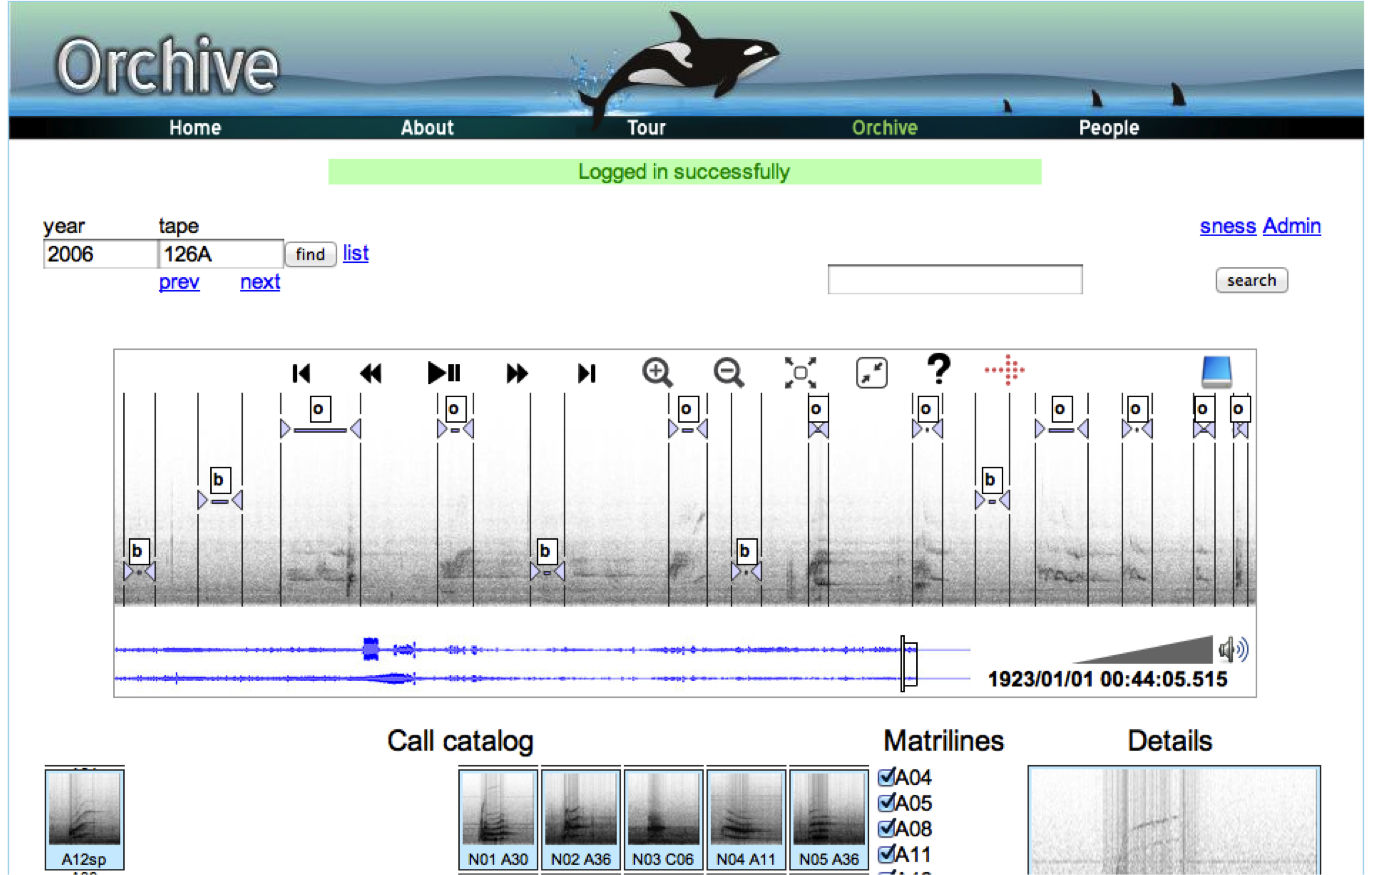
\includegraphics[width=\columnwidth]{figures/dm_orchive}
\label{fig:dm_orchive}
\caption{A small annotated section of audio from the Orchive}
\end{figure}

This interface is still in use, and since July 2008, there have been
approximately 3,900 people who have viewed the site with over 10,000
individual visits.  There are 42 scientists registered as users on the
site, and of these, 11 scientists have contributed annotations.  There
are currently over 17,000 annotations in the database, most of which
label if the clip is an orca vocalization or background noise but also
with almost 4000 that contain which type of orca call is being
vocalized.  Some annotations even contain the pod and/or matrilineal
identity of the call.

A version of this web interface was also developed to view the data
from the VENUS \footnote{\url{http://venus.uvic.ca/}} and
NEPTUNE \footnote{\url{http://www.neptunecanada.com/}} projects.
Dr. Richard Dewey, an Associate Director of VENUS was able to use this
web interface to find the first examples of whale vocalizations in the
VENUS database.  The existing VENUS interface allowed users to only
see one small 5 minute chunk of data at a time, and because the
spectrograms were not precalculated, it took considerable time for
each new 5 minute section of audio to load.  Our system allowed him to
quickly scan over large numbers of recordings to find whale
vocalizations for the first time in the VENUS data.

Even though the interface was in some ways successful, over the years
many drawbacks to this system were identified as people used the
interface and new features were added to the site.

The primary deficiency was that this system required all the
spectrograms and waveform images to be precalculated.  Although this
allowed for a substantially more responsive interface, as new
recordings were added to the database, the entire precalculation
process needed to be repeated.  The last rebuild of these images took
over 3 months of continuous processing time on the server.  Another
downside is the large amount of disk space required to store the
spectrogram images, at the current time, these images take up over 1TB
of disk space for {\diskSpaceOrchive} of audio data.

Another issue with this system is that over time, it became apparent
that there were a number of problematic issues with the software tools
used to create the system.  Even though RoR is still widely used,
there are a number of issues with the performance of the Ruby
language, especially when doing other tasks than simply serving web
pages.  In addition, because of its relative obscurity, there are
issues with APIs for interfacing Ruby to other tools.  It was found
that the Python language has better interfaces to other tools, such as
\textit{Marsyas}, so much of the new code was written in Python.  This allowed
for easier development of new features but increased the number of
languages required to be used, which complicated development time.

In addition, over time the popularity of the Flash platform declined
dramatically, both in terms of acceptance and use by the general
public as well as within the web programming community.  The fact that
Flash could not be used on Apples
iOS \footnote{\url{https://developer.apple.com/devcenter/ios/index.action}}
devices was one of the contributing factors, but the larger factor was
the development of standards-based web interfaces that are not
controlled by a single company but are formed from a consensus among
members of the community.  Because of this, new development on the
site has been done in Javascript.  For example, the call catalog was
developed as a Javascript application.  Interaction between Javascript
applications on the page was straightforward, but interactions between
the main ``orcaannotator'' Flash application and Javascript were often
challenging and became more so as the complexity of the application
grew.

For many tasks in the Orchive, it was found that neither Python nor
Ruby was fast enough, and certain aspects of the site were written in
C++.  For example, the programs to do the calculation of spectrograms
was written in C++ as even in C++ the calculation of all the
spectrograms on the V1.0 website took approximately 3 months on an 8
core machine.

In the end, it became very difficult to add new features to the
website because of the need for development to occur simultaneously in
Ruby, Python, Flash (HaXe), Javascript and C++.  At the current time,
the Orchive version 1 website contains 11,296 lines of Ruby, 3949
lines of HaXe, 987 lines of Javascript, 3405 lines of Python and 2520
lines of C++.  The number of lines of code was manageable, but the
number of languages required to add new features became difficult to
manage.

One big issue that was identified later in the project was that many
of the scientists who would like to participate in the project were in
remote locations with limited or no internet access.  For example,
some of the scientists had limited time to work on annotating data
when in their offices and had more time when they were on board boats
studying orcas.  With the traditional AJAX development paradigm of
having a thin client and most of the code being on the server, the
assumption is that the client has continuous access to a high-speed
internet connection.

Another issue with the website is that in order to support a wide
variety of annotations, it was decided early on to have annotations be
in a free-form text field.  The hope was that scientists would develop
their own consistent vocabulary of annotations and that an open system
for annotations would allow for both a standard vocabulary, for
example, the call types from John Ford's call catalog
\cite{ford1987catalogue}, as well as being flexible enough to
accommodate new annotations.  In a number of ways this was successful,
many of the annotations are in a consistent format.  There are a
number of interesting annotations that would have not been supported
by a fixed vocabulary like ``amazing sequence'' and ``great N4''.
However, the lack of a consistent vocabulary became a major hurdle
when trying to convert these annotations into a form usable by a
machine learning system.  For example, there are 383 ``N1''
annotations, 59 ``N01'' annotations and 20 annotations that contain
either ``N1'' or ``N01'' within them, sometimes preceded by a space or
appended with the matriline or a note about the call.  Writing scripts
to convert these into a consistent vocabulary became progressively
more difficult.

For these reasons, amongst others, it was determined that a new
version of the website should be built using more modern technology
and using a smaller number of programming languages and tools.

\section{orchive v2.0}
\label{section:softwareAndSystems:orchiveV2}

In 2012, a new version of the Orchive software was started from
scratch.  For this new version, it was determined that the Python and
Javascript (Node.js) programming languages would be used for the
server.  Javascript and HTML5 would be used for all client facing
software, and C++ should be used where needed for doing processing of
large datasets on the server.  This allowed us to concentrate
development in Python and Javascript, which greatly simplified
development.

There were a large number of web server platforms available that were
written in Python, and after extensive research and testing, it was
determined that Django provided a good blend between power, popularity
and ease of development.  A subset of this system was also written in
Javascript using Node.js.  The development experience with Node.js was
excellent, it has a new programming paradigm that is ideal for web
based applications, and while it is de facto on the client, it is now
becoming more popular on the server.  It is powerful and fast to
develop in, and is very efficient in terms of resource usage.
However, it is still very much a work in progress; no great
client/server ORM layer could be found that modeled our data well and
linking it to \textit{Marsyas} would have required substantial work.  For
expediency I therefore chose to write the reference
implementation in Django with plans to move the REST API to Node.js at
the earliest opportunity in future work.

I implemented the new spectrogram viewing and audio filtering by by
making a new view in the Django code, and in this view, a \textit{Marsyas}
network is created that calculates a spectrogram and delivers it to
the user with the correct content type.  This functionality of
embedding \textit{Marsyas} directly in the webserver has sped up development of
new audio features considerably.  As some of these audio features are
costly to calculate in terms of processing time, the built in caching
layer in Django is used with Memcached and Apache to cache
spectrograms and other derived audio data.  One should also take into
account that caching may happen at other network layers along the path
to the client, and finally the resources could be cached by the users
browser.

For the front-end, the existence of new tools and frameworks for
developing rich Javascript made it feasible to write larger and richer
web applications.  One of these was the Backbone framework, a toolkit
that allowed for the development of MVC (Model/View/Controller)
applications in Javascript on the client which allowed for the
creation of applications that could work well both in environments
with a high-speed internet connection as well as situations with only
periodic access to the internet.  One of the exciting things about
this kind of framework is that it allowed for the development of
mostly offline applications that could be deployed as tablet or phone
based applications using
PhoneGap \footnote{\url{http://phonegap.com/}}, a framework that
allows developers to build iOS or Android apps using HTML5 and
Javascript.

In addition, the standardization and wide deployment of HTML5 audio in
both the Audio DOM (Document Object Model) element as well as the Web
Audio API made it possible to develop applications that could reliably
play back sound, a vital part of our application.

One of the big issues with the first version of the Orchive software
was the choice to allow for free-form input of annotations by
scientists.  In the new system, I changed this to only allow
annotations from a fixed vocabulary.  However, the system supports an
arbitrary number of such vocabularies, and researchers can add new
entries to these dictionaries.  To support the previously allowed free
form annotations, I added a comment field to the annotation which can
contain whatever text the researcher desires.

Another issue that I came across with the first version of the
website was the need for all the spectrograms, waveforms and other
assets to be pre-generated.  In order to overcome this, I took
advantage of the \textit{Marsyas} bindings to Python and wrote code to allow
the web server to generate spectrograms from audio on the fly.  In
order to improve latency, the Javascript interface sends multiple
requests for rectangular sections of the visible spectrogram, which
allows multiple cores on the server to generate spectrograms in
parallel.  In addition, these spectrograms are cached in memory on the
server (using memcached) to speed up subsequent requests for the same
region of a spectrogram.

Although not all the features of the old site are yet supported in the
new site, the majority of them are, and the new site contains
functionality to display audio features not present in the old site.
There are 2849 lines of Python code in the new interface and 4230
lines of Javascript, which shows the dramatic move from a server-based
application to a client-based application.

Although both versions of the website use a REST (Representational
State Transfer) based API \cite{fieldingphd}, the new Javascript code
uses this REST API exclusively for communication of state between the
server and client.

In order to deal with the issue that the code had to be cloned for
different projects, the new version of the website allows for multiple
projects to co-exist within one set of web server code.  Currently, the
system contains three different projects, the Orchive, a site with
bird bioacoustic data from the Alberta Biodiversity Monitoring
Institute and a project dealing with partially annotated chant data
from the Torah and Koran traditions.  Because of this, bug fixes and
updates made to one project are reflected in all the other projects.
The web server displays different headers and graphics for the
different projects and supports different domain name URLs to access
the data, which allows the different projects to maintain their
identity.

For a system diagram of how this process of machine learning, expert
interfaces and serious casual games works, refer to Figure
\ref{fig:systemDiagram}.

\begin{figure}
\centering
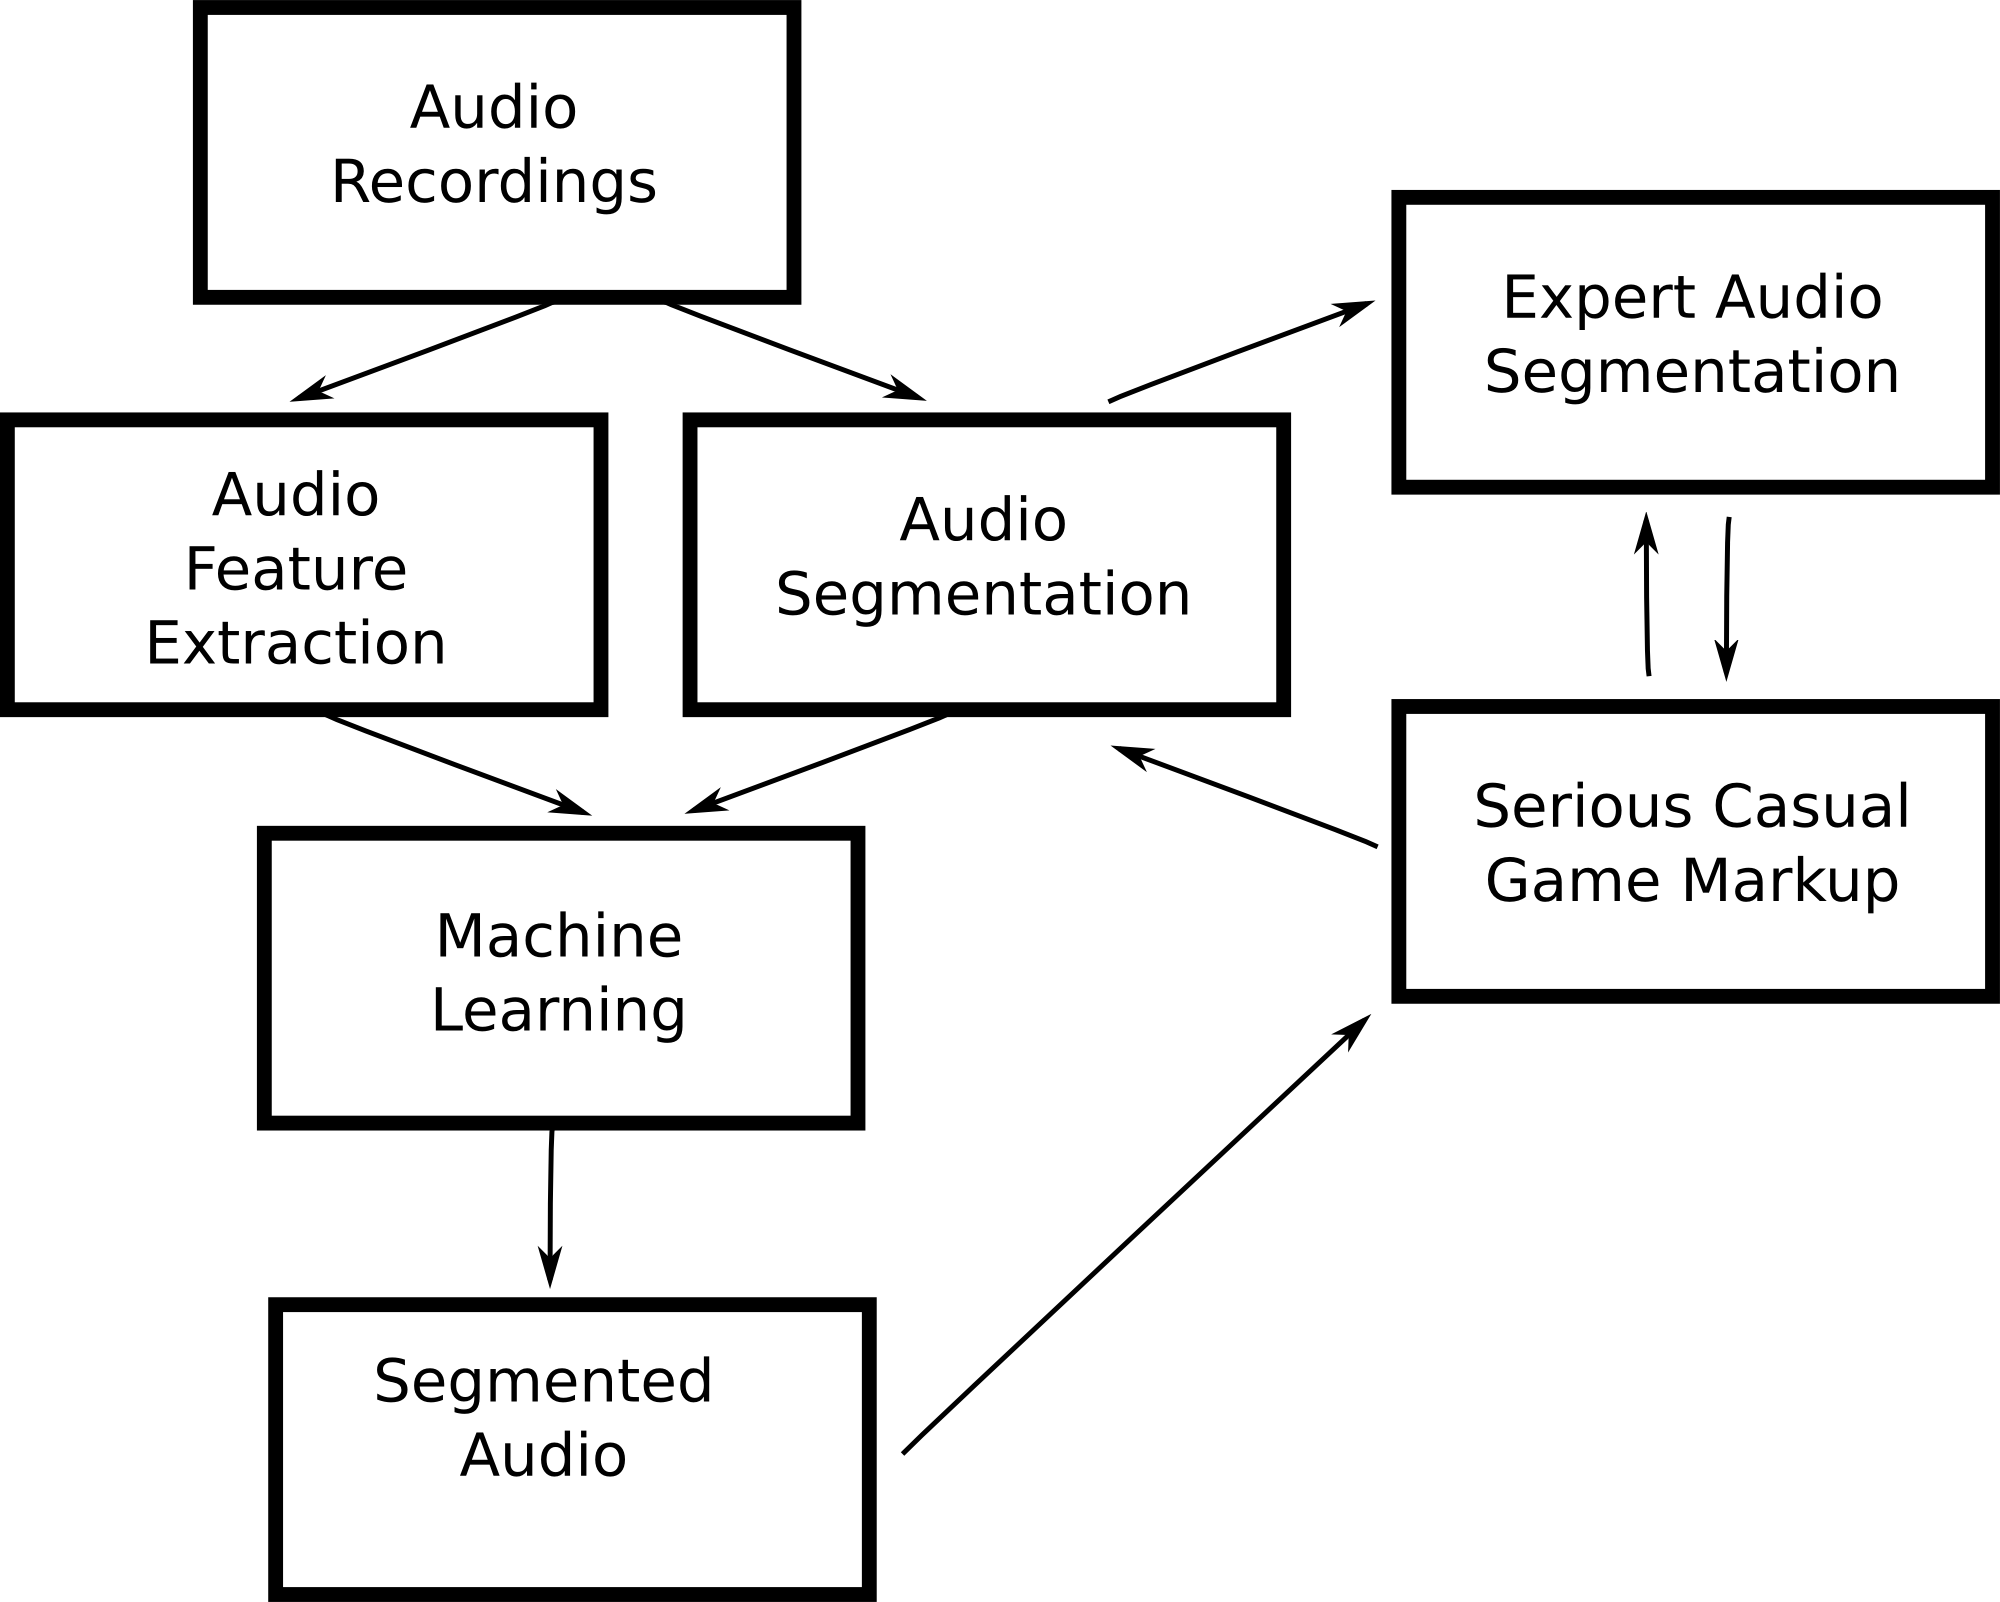
\includegraphics[width=80mm]{figures/systemDiagram}
\caption{A high level overview of the system in the Orchive.  The
  audio recordings are the main input to the system, these undergo
  processes of audio feature extraction concurrently with audio
  segmentation by a machine learning system.  this roughly segmented
  audio can be further refined in the expert audio segmentation
  process which can interact with a serious casual game markup system
  to label audio clips along with a machine learning system.}
\label{fig:systemDiagram} 
\end{figure} 


\subsection{Recording View}

Like in Orchive V1.0, the Recording View is designed to be the main
view that the user interacts with, and can be seen in Figure
\ref{fig:orchiveV2recording}.  At the top of the screen is a header
that has links to the various tools available, look at and annotate
the Recordings, build Training Sets from the annotated Recordings,
train Classifiers on the Training Sets and look at the Predictions of
Classifiers on Recordings.  In the middle of the screen is a
spectrogram view of the sound, with shuttle controls above it to
control the playback of sound.  One feature that was asked for many
times by biologists using orchive v1.0 was to have a frequency scale on
the left hand side, this was added in the new version.

On this spectrogram six clips can be seen, the first three of
``orca'', and the last three of ``background''.  Like in the V1.0
interface, these clips can be adjusted to more accurately annotate the
sound under interest.

Below these clips is the new Clip Catalog.  In V2.0, once one selects
a region of audio, the expert user assigns it a label by either
clicking on one of the items in the call catalog, or by typing a
number from 1-9 that corresponds to the number of the call in the
catalog.  This addition of a call catalog greatly simplifies the
process of training machine learning classifiers and building game
levels, as their vocabulary is fixed.  To the right side of the call
catalog is a control to select different call catalog entries, and a
detailed view of the currently selected call below.  On the far right
side is a list of the prediction runs using a machine learning
classifier that have been done for this recording.  The third one of
these has been clicked, and this in turn has displayed a blue overlay
on the spectrogram for regions classified as ``orca'', a green overlay
for ``voice'' and transparent for ``background''.

It was challenging to transition the old free annotations to the new
fixed vocabulary system.  A series of scripts was developed that
implemented a set of heuristics to turn call types like ``n1'', ``N1'',
``N01'' and ``A04 N01'' into it's corresponding canonical label which
was of the form ``N01''.

\begin{figure}[t]
\centering
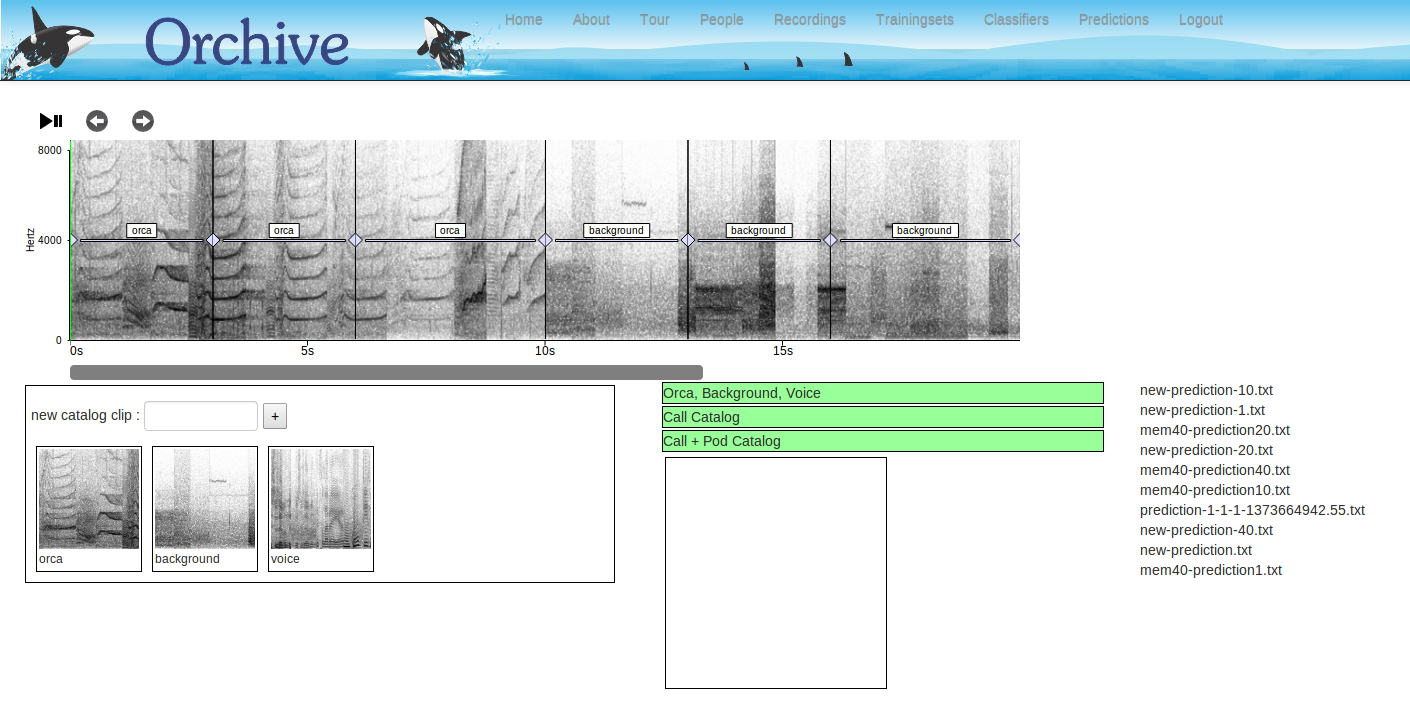
\includegraphics[width=\columnwidth]{figures/orchiveV2recording}
\label{fig:orchiveV2recording}
\caption{Recording View - A picture showing the main recording view of
the orchive v2.0.  In the middle of the screen is the main spectrogram,
which is calculated on the fly and loaded in chunks to improve the
user experience.}
\end{figure}


\subsection{Training Set View}

One of the most challenging parts of dealing with the huge datasets
that are associated with large bioacoustic archives is building the
training and testing sets of data which are used by audio feature
extraction and machine learning algorithms.  One needs to search for
the right clips, to listen to and see them, and to sort them according
to different criteria as was done using
another Flash based interface I previously wrote called Cantillion
\cite{biro2012computational}.  The Training Set View, show in Figure
\ref{fig:orchiveV2trainingset} implements this functionality in the
orchive v2.0 interface.

\begin{figure}[t]
\centering
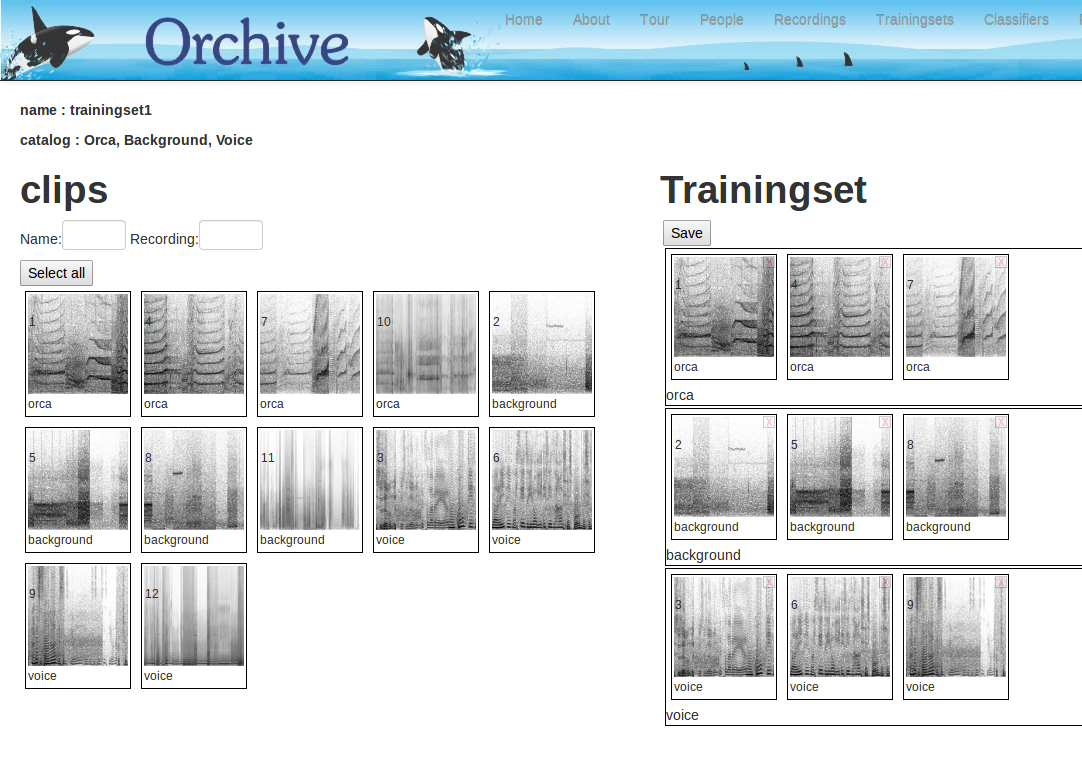
\includegraphics[width=\columnwidth]{figures/orchiveV2trainingset}
\label{fig:orchiveV2trainingset}
\caption{Training Set - A screenshot of the interface to allow
  researchers to manually create training and testing sets of data
  directly from the annotated clips in the archive.  On the left is
  the call catalog, and on the right are boxes for the different
  classes in the training set that is being constructed.}
\end{figure}



On the left hand side, a set of clips that correspond to the currently
selected search parameters are displayed.  To filter for clips with a
specific name, one would type the name in the ``Name'' field, and to
filter by recording, in the ``Recording'' field.  These clips can be
seen, can be clicked on to hear them, and if they are appropriate, can be
dragged to the Trainingset box on the right.  Each of the bins
represents a different label, and by dragging a clip to one of these
bins, a new clip is added to the training set with that label.

In actual use however, it seems the primary way of creating new
training sets was from the main training set page, where all
appropriate clips in the entire dataset will be used.  However, this
interface will still be useful when examining training sets or
building small, custom training sets.


\subsection{Data View}

\begin{figure}[t]
\centering
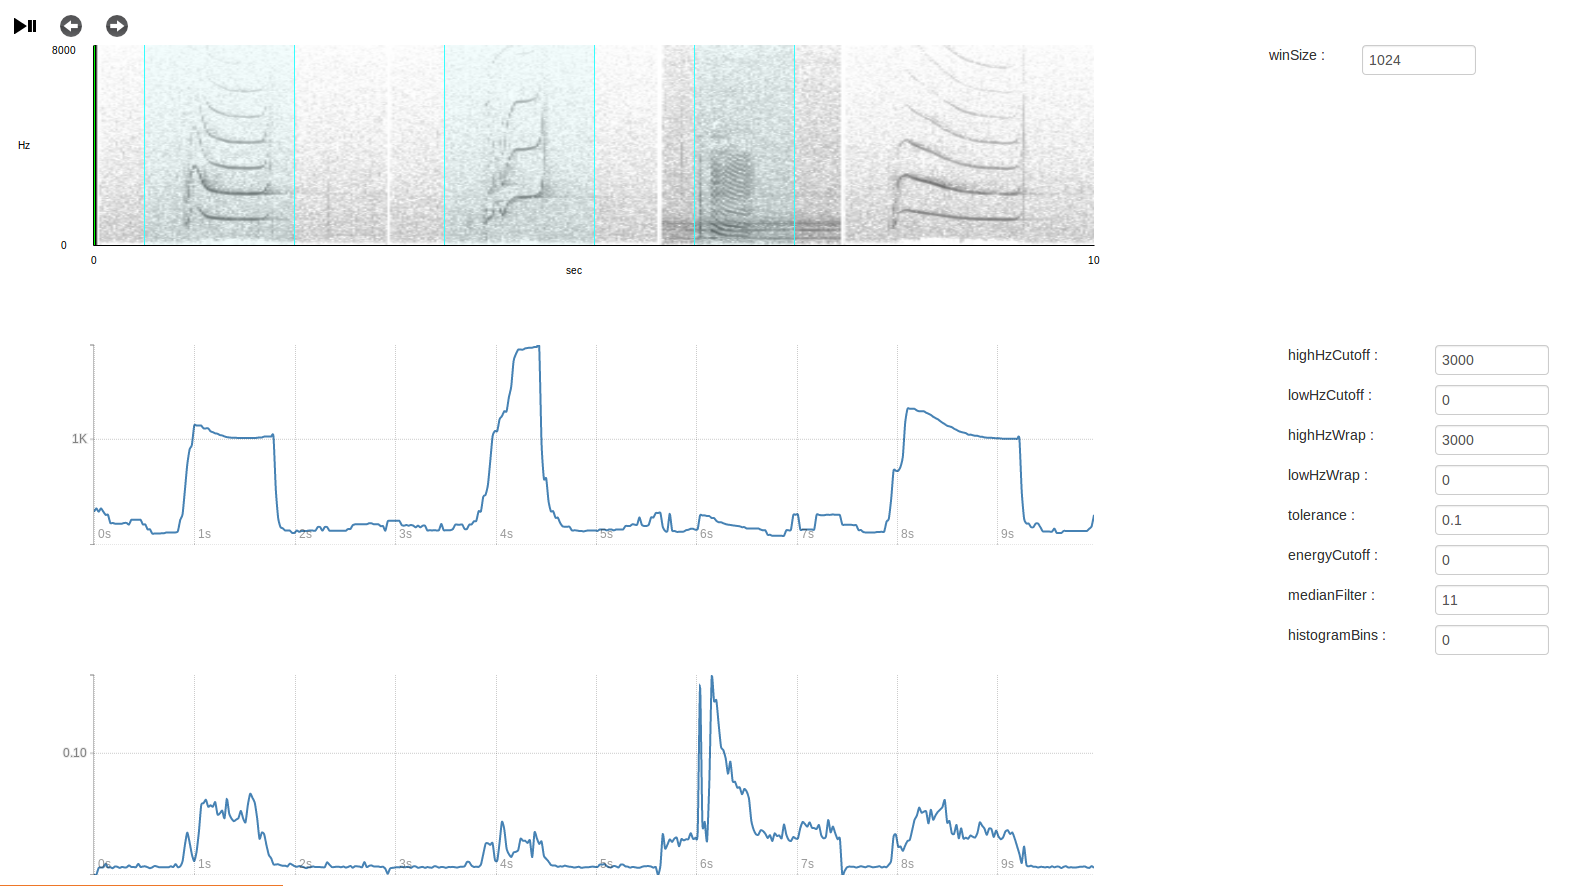
\includegraphics[width=\columnwidth]{figures/orchiveV2dataView}
\label{fig:orchiveV2dataView}
\caption{A screenshot of the data viewer for the Orchive, showing a
  test section of audio with four orca calls from the call catalog.
  At the bottom is a graph of the output of the YIN pitch
  determination algorithm, and below that is the RMS energy of the
  signal.}
\end{figure}

In order to tune the audio features that are calculated for
bioacoustic data, it is useful to be able to see a graphical
representation of the audio data.  The Data View, shown in Figure
\ref{fig:orchiveV2dataView} provides this functionality.  The data
view uses a similar plugin structure to that used in the main
recording view, and the two can coordinate with each other through
Backbone so that when the scrollbar of one component is moved, the
other follows along.  This shows the power of this Javascript plugin
component method, where a central Backbone core connects a wide
variety of rich web interfaces, some custom, like the ones discussed
here, and others that can come from a wide variety of open and closed
source vendors.


\subsection{Game Builder View}

Once clips have been created in the Recording View, they can then be
used to create citizen science games.  The goal of these citizen
science games are to collect more data from more people than is
possible using the limited number of experts in orca vocalizations
that are available.  In the first version of the game, the interface
to add new levels was text-based and was not able to be used by the
primary stakeholders at OrcaLab which turned out to be an important
feature.  In game design, it is important to have a balance of fun and
difficulty to interest people in the game, especially in the early,
training levels.  Stakeholders at OrcaLab and other expert scientists
who played the game gave copious amounts of feedback over the exact
choice of call types in each of the levels.  In one case, one of the
experts in orca call recognition sent us a detailed list of the issues
with the current game levels that was over one thousand words long.
This could be an unexpected way to enlist the assistance of
biologists, to get them to help to design new game levels.  This would
give us additional expert labeled clips when they design the game
level, and could be used to give us citizen science data as well.
Because of these many factors, it was decided to build a new interface
to allow the bespoke construction of new levels.

In order to fufill these requirements, an editor for creating and
editing game levels was developed.  In this editor, a call catalog
like the one seen above in the training set view can be seen on the
left.  On the right is a series of boxes, each which corresponds to a
level.  In the first box, the game designer puts the query call, then
the correct call, and then four other incorrect call types.  The
functionality that this interface provides was essential in order to
allow for the collaboration on making game levels with our partners.
However, for most of the use of the citizen science game, the levels
are constructed automatically by the computer to classify new clips.
In this case, the entire call catalog is displayed to the user along
with the four most likely call types.

\begin{figure}[t]
\centering
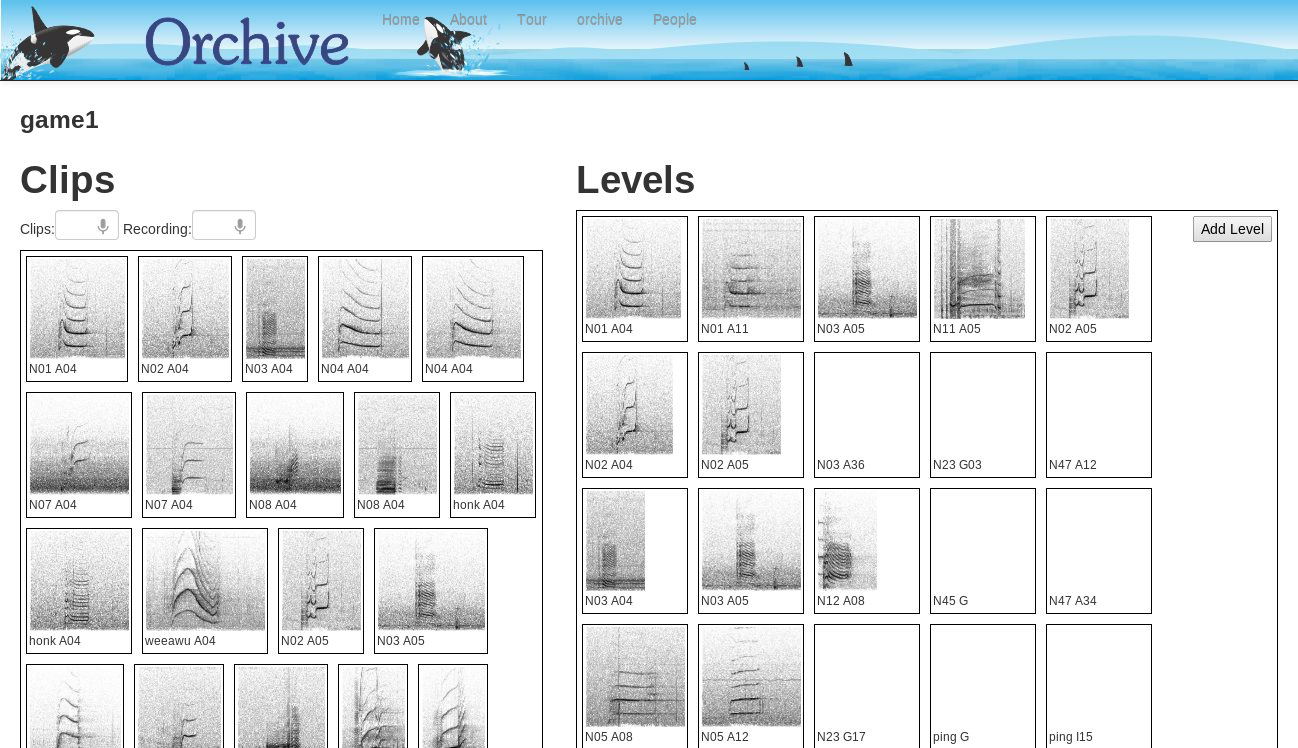
\includegraphics[width=\columnwidth]{figures/orchiveV2gameBuilder}
\label{fig:orchiveV2gameBuilder}
\caption{A screenshot of the interface by which researchers can
  construct new custom levels of the OrcaGame using a web browser.
  All the annotations in the database are able to be added to the
  interface by the researcher, who can quickly build new levels to
  test the skill level of users.}
\end{figure}

\subsection{Citizen Science Game}

A view of the main play screen in the citizen science game can be seen
in Figure \ref{fig:OrcaGame}.  At the top of the screen is the Query
clip, and below are the Reference clips.  The user can click on the
clips and they will make their corresponding sound.  When they are
satisfied with their decision, they press the ``Select'' button and a
message telling them if they are correct or incorrect is shown.

\begin{figure}[h]
\centering
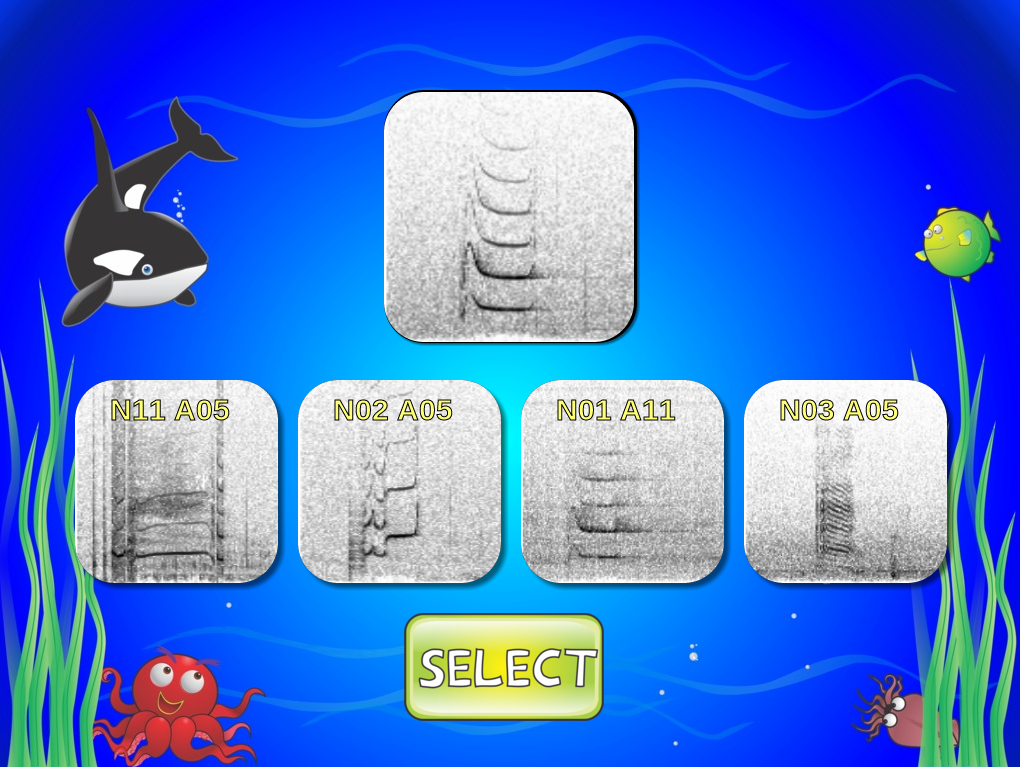
\includegraphics[width=\columnwidth]{figures/orcagame}
\caption{A screenshot of the OrcaGame interface, showing the query
  call at the top of the screen and the the reference call types below.}
\label{fig:OrcaGame}
\end{figure}

\section{Distributed Computing}
With the huge sizes of datasets in large bioacoustic archives,
computing audio features and running machine learning tasks on the
entire archive requires the use of clusters of large numbers of
machines.  In this thesis, the Westgrid collection of computational
clusters is used for running the huge audio feature extraction and
machine learning task. This uses a very simple queuing system known as
Torque \footnote{\url{http://www.adaptivecomputing.com/products/open-source/torque/}},
which is the latest evolution of the ancient PBS
\cite{henderson1995job} (Parallel Batch System) parallel job
distribution system. PBS allows scientific users to schedule large
jobs to run on computers, and performs well for certain scientific
tasks where a single, usually large, program is run on a variety of
different datasets, and the results are then saved to disk and later
analyzed by a scientist. This type of computing is now known as Grid
Computing.  While this system has certain benefits for running
specific scientific tasks, for other tasks, the methodology of having
separate computers running mostly independently, and all coordination
of tasks being the responsibility of the programmer with a tool such
as MPI quickly becomes difficult. The MapReduce paradigm helps in the
coordination of large parallel tasks, and the Hadoop system allows
programmers to efficiently write distributed programs that run on huge
numbers of computers and allows for failures of individual computers.

\section{Summary}

The system and software developed for this thesis was an integral part
of the preparation of training and test sets for the machine learning
section of the thesis.  It was also essential for the data collection
from biologists and formed the interface by which data was collected
from both biologists and citizen scientists.  It currently stores
approximately \aboutHoursOfOrchiveRecordings hours of audio and is in
active use by the public and by researchers in orca vocalizations.
For these reasons, it is important that the software and its design be
considered as an important part of this thesis, and the part that took
the majority of the time spent.

Two slightly different architectures were used with different choices
of programming languages for version 1.0 and version 2.0 of the
Orchive.  For the first version, a gradual drift in technology made it
necessary to support a complex system that used five different
programming languages and required client side interaction between
Flash and Javascript to provide for rich interfaces.  Other features
were changed for version 2.0 from lessons learned on version 1.0 and
detailed above.  This new interface is live and can be seen at the Orchive
website
\footnote{\url{http://orchive.net}}.

In the following sections, data taken from all orca vocalization
experts from orchive v1.0 was taken as input, this gave a total of
\totalAnnotations clips.  This data was then taken as input into
Version 2.0 of the Orchive interface and was cleaned by removing
regions of silence before and after the clip.  Clips that did not
appear on quick visual and auditory inspection to have orca
vocalizations in them were removed.  Subsequent investigation of these
revealed that in many cases these were just the vocalizations of
extremely distant orcas; however, they were still not used in the
results presented due to the uncertainty of the experimenter in their
validity.  Work on the ABMI project has shown the extreme importance
of having trained listeners as it appears trained listeners can hear
many times more distant birds than untrained listeners.  Although
other interfaces could have been used to annotate this audio, this
custom built interface allowed for the easy collating of results from
diverse sources and for trimming their audio for input to machine
learning algorithms.

The field of CSCW \cite{bannon1991cscw} deals with making tools to
deal with problems like this, in which large amounts of data must be
interacted with by multiple communities of users in order to create
knowledge.  The system that was built for this thesis takes
inspiration from many different CSCW systems to build a tool that
multiple groups of people can use to solve large bioacoustic problems.
This system was essential in the creation the large datasets that were
used in the evaluation of this system in Chapter \ref{chap:evaluation}
which examines if the approach hypothesized in this paper is an
effective way to annotate large bioacoustic archives.

